\documentclass[12pt]{amsart}

\usepackage[margin=1in]{geometry}
\usepackage{amsmath}
\usepackage{amssymb}
\usepackage{amsthm}
\usepackage{setspace}
\usepackage{graphicx}
\usepackage{subfig}
\usepackage{url}
\usepackage{algorithm}
\usepackage{algpseudocode}
\usepackage{placeins}

\author{David~Love and G\"{u}zin~Bayraksan}

\title{A Likelihood Robust Method for Water Allocation under Uncertainty}
\date{}

% Frequently used general mathematics
\newcommand{\R}{{\mathbb{R}}}
\newcommand{\Rp}{\R^+}
\newcommand{\Z}{{\mathbb{Z}}}
\newcommand{\Zp}{\Z^+}
\newcommand{\Q}{\mathbb{Q}}
\newcommand{\N}{\mathbb{N}}

% Commands for probability
\renewcommand{\P}{\mathbb{P}}
\newcommand{\p}[1]{\P \left[ #1 \right]}
\newcommand{\e}[1]{\mathbb{E} \left[ #1 \right]}
\newcommand{\ee}[2]{\mathbb{E}_{#1} \left[ #2 \right]}

% Definitions of variables
\newcommand{\X}{X}
\newcommand{\x}{\mathbf{x}}
\newcommand{\xh}{\hat{\x}}
\newcommand{\lh}{\hat{\lambda}}
\newcommand{\mh}{\hat{\mu}}
\newcommand{\xs}{\x^*}
\newcommand{\xit}{\tilde{\mathbf{\xi}}}
\newcommand{\zt}{\tilde{z}}
\newcommand{\zs}{z^*}

% Further variables
\newcommand{\y}{\mathbf{y}}
\renewcommand{\c}{\mathbf{c}}
\newcommand{\q}{\mathbf{q}}
\renewcommand{\b}{\mathbf{b}}
\renewcommand{\d}{\mathbf{d}}

% Useful mathematics functions
\DeclareMathOperator*{\argmin}{argmin}
\newtheorem{theorem}{Theorem}
\newtheorem{lemma}[theorem]{Lemma}
\newtheorem{proposition}[theorem]{Proposition}
\newtheorem{corollary}[theorem]{Corollary}
\newtheorem{definition}[theorem]{Definition}
\newcommand{\st}{\mbox{s.t.}}

\begin{document}

\begin{titlepage}
\begin{center}

\vspace*{4cm}

% Title
{ \huge A Data-Driven Method for\medskip\\ Robust Water Allocation under Uncertainty}\\%[0.4cm]

\vspace{3cm}

\begin{minipage}{0.45\textwidth}
\begin{flushleft} \large
\emph{Fellow:}\\
 David \textsc{Love}\\
 Interdisciplinary Program in Applied Mathematics\\
 University of Arizona
\end{flushleft}
\end{minipage}
\begin{minipage}{0.45\textwidth}
\begin{flushright} \large
\emph{Adviser:} \\
 Dr.~G\"{u}zin \textsc{Bayraksan}\\
 Integrated Systems Engineering\\
 The Ohio State University, and\\
 Systems \& Industrial Engineering\\
 University of Arizona
\end{flushright}
\end{minipage}

\vspace{2cm}

{\large May 10, 2012}

\vspace{2cm}

% Bottom of the page
{\large University of Arizona, Technology and Research Initiative Fund 2012/2013\\Water Sustainability Graduate Student Fellowship Program}

\end{center}
\end{titlepage}

\section{Arizona water issue addressed}

More than 25 million people in the southwestern United States depend on the water supplied by the Lower Colorado River Basin for their livelihood.
More than half of Tucson's water, for instance, comes from this source.
The Colorado River Basin has experienced a sustained period of drought in recent years, which has led to questions about the adequacy of the Colorado to meet future demands, especially as the population of Arizona (and of other states that depend on this water source) increases.
Thus, the problem of allocating Colorado water is of critical importance. 

%The southeastern portion of Tucson shown in Figure \ref{fig:tucson_map} is a newly developing area and is expected to grow considerably. 
%The LRLP-2 water allocation model would help authorities with future water plans in this area while being robust to uncertainties in water supplies and demands.

In this work, we model, solve, and analyze a robust water allocation problem to optimally allocate Colorado River water to different users over 40 years in the southeastern part of Tucson.
There are many uncertainties in this water allocation problem---two of most important ones are water supply and water demands.  
On the water demand side, the southeastern portion of Tucson is expected to grow  during the time horizon considered; therefore, the water demand is expected to increase but by how much is uncertain. 
On the water supply side, it is well recognized that the reliability of the Colorado River system under future climate variability is critically important to the long-term well-being of Arizona and the other six states that depend on this water supply \cite{usbr_colorado_climate}. 
The current approach of estimating water supply using climate models is to use Global Circulation Models (GCM) to generate regional rainfall and temperature scenarios by the so-called statistical downscaling techniques \cite{christensen_lettenmaier_07,dibike_caulibaly_05}. 
Even though we have some idea about these uncertainties, there is considerable ambiguity as to how to model these uncertainties and how to make long-term decisions under such ambiguous uncertainties. 
The work presented here aims to tackle this important question applies it to a water allocation problem in Tucson, AZ. 
This would help authorities with future water plans in this area of Tucson while being robust to uncertainties in water supplies and demands.


Our methodology uses a generalized network model of Colorado River water allocation in Tucson, Arizona motivated by the CALVIN (CALifornia Value Integrated Network) optimal water allocation model of California created by Draper et al.\ \cite{draper_etal_03}.
More general models of Colorado River water distribution have also been studied, such as the Colorado River Reservoir Model \cite{christensen2004effects} and the Colorado River Budget Model \cite{barnett2009sustainable}.
Our model is modified to incorporate ambiguous future uncertainty by using the {\it Likelihood Robust Optimization (LRO)} approach of Wang, Glynn and Ye \cite{wang2010likelihood}.


LRO is a data-driven method that uses observations of random or unknown parameters to account not only for inherent stochasticity of a problem, but the uncertainty of the probabilistic model itself.
This is especially important in our application as we are looking 40 years into the future and there is considerable ambiguity in the uncertainties.
The LRO is especially attractive because only those scenarios of interest, obtained either through observation or simulation, are used directly in the calculations.
The size of the problem is polynomial in the number of scenarios used, making it computationally tractable.
Furthermore, the scenarios used in the LRO can represent select ones that are of interest to the authorities. 
For instance, the US Bureau of Reclamation uses an approach called the {\it scenario planning} that examines water demand and supply scenarios over the next 50 years \cite{usbr_11}.  
Similar studies are being conducted by Tucson Water  \cite{cityofTucsonWaterPlan}.
%LRO fits this practice well because the scenario planning process results in several scenarios that the agencies would especially like to be robust against.


In this report, we first discuss the methods use in Section \ref{sec:methods}, and point out some key results in Section \ref{sec:results}.
Any figures and tables mentioned are included in the appendix.
We end with a short summary and future work.



%%%%%%%%%%%%%%%%%%%%%%%%%%%%%%%%%%%%%%%%%%%%%%%%%%%%%%%%%%%%%%%%%%%%%%%%%%%%%%%%
\section{Methods}
\label{sec:methods}

\subsection{Generalized Network Water Model} 
\label{sec:network_model}

We begin with a multi-period generalized network flow model of Colorado River water allocation in southeastern Tucson, shown in Figure \ref{fig:tucson_map}.
The generalized network model is defined by a set of nodes and directed arcs $(N,\: A)$.
The nodes $N$ represent available water supply from the Colorado River, water treatment plants, reservoirs, and water demand sites.
The arcs $A$ represent the conveyance system (pipes, etc.) that carry water between the nodes.
Figures \ref{fig:nodes_central}, \ref{fig:zones_c_e}, and \ref{fig:zones_split} show the layout of the water distribution model.
Water can be stored in between time periods in reservoirs to meet future demands.
The model aims to find the minimal cost water flows considering energy, treatment, storage, and transportation costs over the planning period. 
In addition, the model contains penalty costs for unmet demands. 
Generalized network water allocation models have been used to find water allocations and delivery reliabilities and to assess values of different water use operations; see, e.g., \cite{draper_etal_03}. 

Water flows on arc $(i,j) \in A$ during time period $t = 1, \dots, P$ are represented by decisions $x_{ijt}$.
Each arc $(i,j) \in A$ and time period $t$ has a unit cost $c_{ijt}^x$, loss coefficient $0 \leq a_{ijt} \leq 1$ to account for evaporation, leakage from the pipes, etc., and bounds on the flow $l_{ijt}^x \leq x_{ijt} \leq u_{ijt}^x$.
Each node $j \in N$ has a supply/demand for time period $t$, denoted by $b_{jt}$.
Nodes representing reservoirs are able to store water between time periods.
Stored water available at node $j$ at the beginning of time period $t$ is $s_{jt}$, with associated storage cost $c_{jt}^s$ and bounds $l_{jt}^s \leq s_{jt} \leq u_{jt}^s$.
Finally, water released into the environment from node $j$ in period $t$ is given by $r_{jt}$, with bounds $l_{jt}^r \leq r_{jt} \leq u_{jt}^r$.
The deterministic model is a multi-period generalized network flow model of the form
\begin{align*}
	\min_{x,s,r} \ & \sum_{(i,j) \in A} \sum_{t=1}^P c_{ijt}^x x_{ijt} + \sum_{j \in N} \sum_{t=1}^P c_{jt}^s s_{jt}\\
	\st \ & \sum_{i \in N} x_{jit} + s_{j,t+1} + r_{jt} = \sum_{i \in N} a_{ijt} x_{ijt} + s_{jt} + b_{jt}, \ \ \forall j,t \\
	& l_{ijt}^x \leq x_{ijt} \leq u_{ijt}^x,\ \ \ \forall i,j,t \\
	& l_{jt}^s \leq\ s_{jt}\  \leq u_{sjt}^s, \ \ \ \forall j,t \\
	& l_{jt}^r \leq\ r_{jt}\  \leq u_{sjt}^r, \ \ \ \forall j,t.
\end{align*}


In practice, many parameters are unknown, especially as we further look into the future. 
This is particularly true of the water supply and demands, denoted by $b_{jt}$ in the above model. 
To capture this uncertainty, we first make this model stochastic by rewriting it as a two-stage linear program.
Later, we will modify this model to be robust against all future scenarios considered in the next subsection. 
The model has a total of $P$ time periods, which is split into two stages of $P_1$ and $P_2 = P - P_1$ years each. 
The water supplies and demands $b_{jt}$ are assumed to be known during the first stage of $P_1$ years and in the remaining $P_2$ years, they are uncertain and modeled using a discrete set of scenarios with a specific probability distribution.  
Note that we also assume some lower and upper bounds to be stochastic in the second stage. 

The two-stage stochastic model allocates water at a minimal cost in the first stage and in the second stage, it tries to minimize the total expected cost given the first-stage decisions.   
The model thus becomes
\begin{align}
	\min_{(x,s,r) \in L^1} \ & \sum_{(i,j) \in A} \sum_{t=1}^{P_1} c_{ijt}^x x_{ijt} + \sum_{j \in N} \sum_{t=1}^{P_1} c_{jt}^s s_{jt} + \sum_{\omega=1}^n p_\omega h^\dagger_\omega(s) \label{eq:gen_network_two_stage} \\
	\st \ & \sum_{i \in N} x_{jit} + s_{j,t+1} + r_{jt} = \sum_{i \in N} a_{ijt} x_{ijt} + s_{jt} + b_{jt},\ \ \ \ \forall j, 1 \leq t \leq P_1, \notag
\end{align}
where the $\omega$ index indicates the $n$ second-stage scenarios with probabilities $p_\omega$, the last term in (\ref{eq:gen_network_two_stage}) denotes the expected second-stage costs, which are found by solving the following problems over each scenario $\omega$
\begin{align}
	h^\dagger_\omega(s) = \min_{(x,s,r) \in L^2_\omega} \ & \sum_{(i,j) \in A} \sum_{t=P_1+1}^{P} c_{ijt}^x x_{ijt} + \sum_{j \in N} \sum_{t=P_1+1}^{P} c_{jt}^s s_{jt} \label{eq:gen_network_second_stage} \\
	\st \ & \sum_{i \in N} x_{jit} + s_{j,t+1} + r_{jt} = \sum_{i \in N} a_{ijt} x_{ijt} + s_{jt} + b_{jt}^\omega, \ \ \ \ \forall j, P_1+1 \leq t \leq P, \notag
\end{align}
and $L^1$ and $L^2_\omega$ represent the feasible regions defined by the lower and upper variable bounds.

In the rest of the report, we simplify the notation for the first-stage (\ref{eq:gen_network_two_stage}) and second-stage (\ref{eq:gen_network_second_stage}) problems as follows.
In the first stage, decision variables $\{x_{ijt}\}$, $\{s_{jt}\}$ and $\{r_{jt}\}$ become the vector $\x$, costs $\{c_{ijt}^x\}$ and $\{c_{jt}^s\}$ are written as the row vector $\c$, the supply/demand parameters $b_{jt}$ become the vector $\b$ and the constraint matrix is written as $A$.
In the second stage, we denote the decisions as $\y^\omega$, the costs as $\q^\omega$, the supply/demands as $\d^\omega$, and the constraint matrices multiplying $\y^\omega$ and $\x$ as $D^\omega$ and $B^\omega$, respectively.
This notation puts the generalized network model in the form of a {\it two-stage stochastic linear program with recourse (SLP-2)}, formulated as
\begin{align}
	\min_\x \ & \c\x + \sum_{\omega=1}^n p_\omega h^\dagger(\x) \label{eq:slp_first_stage} \\
	\st \ & A\x = \b \nonumber  \\
	&\ \ \ \x \geq 0 \nonumber
\end{align}
where
\begin{align}
	h^\dagger_\omega(\x) = \min_{y^\omega} \ & \q^\omega y^\omega \label{eq:slp_second_stage} \\
	\st \ & D^\omega y^\omega = B^\omega \x + \d^\omega \nonumber \\
	& \ \ \ y^\omega \geq 0. \nonumber
\end{align}
For simplicity we assume relatively complete recourse; i.e., the second-stage problems $h^\dagger_\omega(\x)$ are feasible for every feasible solution $\x$ of the first-stage problem. In our application, there are penalty costs when demand is not met; therefore, our model has relatively complete recourse. 


%%%%%%%%%%%%%%%%%%%%%%%%%%%%%%%%%%%%%%%%%%%%%%%%%%%%%%%%%%%%%%%%%%%%%%%%%%%%%%%%
\subsection{Robust Water Allocation Formulation}
\label{sec:lrlp2}

The two-stage stochastic formulation, compactly written as SLP-2 above, assumes that the probability of each scenario $\{p_\omega\}_{\omega=1}^{n}$ is known.
However, in many applications, including our water planning, these probabilities are unknown; in other words, the governing probability distribution is unknown.
One technique to deal with this type of uncertainty is to replace the assumed known distribution with an {\it ambiguity set} of distributions; i.e., a set of distributions which is believed to contain the true distribution and to be robust against this set.
In the likelihood robust formulation, we assume scenario $\omega$ has been observed $N_\omega$ times, with $N = \sum_{\omega=1}^n N_\omega$ total observations. 
Note that these observations could represent expert opinions, different simulations of the future, etc. 
If not much is known, each scenario can be taken to be equally likely ($N_\omega = 1$ or equal for all $\omega$) and the robustness level can be adjusted. 
In the stochastic formulation SLP-2, having  $N_\omega$ observations for each scenario $\omega$ would correspond to probability of scenario $\omega$ to be $p_\omega = N_\omega / N$, which is the maximum likelihood distribution. 
The {\it ambiguity set}, however, is defined by the set of distributions with sufficiently high empirical likelihood $\prod_{\omega=1}^n p_\omega^{N_\omega}$. 
By replacing the specific distribution in SLP-2 with a set of distributions with  high empirical likelihood, we create a model that we refer to as {\it two-stage likelihood robust linear program with recourse (LRLP-2)}.

To derive the LRLP-2, we begin by writing SLP-2 given in \eqref{eq:slp_first_stage}--\eqref{eq:slp_second_stage} in extensive form by putting the first and second stages together
\[
	\begin{array}{rrrl}
		\min_{\x,y^\omega} \ & \c\x & + \sum_\omega p_\omega \q^\omega y^\omega \label{eq:slp2cost} \\
		\st \ & A\x & & = \b \nonumber \\
		& -B^\omega \x & + D^\omega y^\omega & = \d^\omega,\ \forall \omega \nonumber \\
		& \x & & \geq 0 \nonumber \\
		& & y^\omega & \geq 0,\ \forall \omega. \nonumber
	\end{array}
\]
The SLP-2 formulation is then augmented by the set of distributions with sufficiently high likelihood.
To be robust against all these possible distributions, the distribution that results in the maximum expected cost is considered.
Then, the objective function is minimized with respect to this worst-case distribution selected from the ambiguity set of distributions.
The resulting minimax formulation of LRLP-2 is
\begin{align}
	\min_{\x,y^\omega} \max_p \ & \c\x + \sum_\omega p_\omega \q^\omega y^\omega \label{eq:lrlp_primal}\\
	\st \ & A\x = \b \nonumber \\
	& -B^\omega \x + D^\omega y^\omega = \d^\omega,\ \forall \omega \nonumber \\
	& \sum_\omega N_\omega \log p_\omega \geq \gamma &   \label{eq:lrlp_primal_liklihood} \\
	& \sum_\omega p_\omega = 1 &   \label{eq:lrlp_primal_probability} \\
	& \x \geq 0 \nonumber \\
	& y^\omega, p_\omega \geq 0,\ \forall \omega. \label{eq:nonneg}
\end{align}
Following Wang et al.\ \cite{wang2010likelihood}, we have introduced the likelihood parameter $\gamma$, and used it to construct the ambiguity set of distributions $\{p_\omega\}_{\omega=1}^{n}$ satisfying constraints (\ref{eq:lrlp_primal_liklihood}), (\ref{eq:lrlp_primal_probability}), and (\ref{eq:nonneg}).
Note the likelihood constraint \eqref{eq:lrlp_primal_liklihood} is equivalent to $\prod_{\omega=1}^n p_\omega^{N_\omega} \geq e^\gamma$, which explicitly states that the empirical likelihood should be above a certain desired level dictated by $e^\gamma$. 
Constraint \eqref{eq:lrlp_primal_probability}, along with nonnegativity constraints on $p_\omega$ given in (\ref{eq:nonneg}), simply ensure that $\{p_\omega\}_{\omega=1}^{n}$ constitutes a probability distribution. 
Let $0 \leq \gamma' \leq 1$ be the \emph{relative likelihood parameter} that expresses $\gamma$ as a {\it proportion} of the maximum likelihood; i.e., $\gamma = \log( \gamma' \prod_\omega (\tfrac{N_\omega}{N})^{N_\omega})$.
When discussing our application and key results in the next section, we will be referring to $\gamma'$.

%%%%%%%%%%%%%%%%%%%%%%%%%%%%%%%%%%%%%%%%%%%%%%%%%%%%%%%%%%%%%%%%%%%%%%%%%%%%%%%%
\section{Key Findings}
\label{sec:results}

%%%%%%%%%%%%%%%%%%%%%%%%%%%%%%%%%%%%%%%%%%%%%%%%%%%%%%%%%%%%%%%%%%%%%%%%%%%%%%%%
\subsection{Application} 
\label{sec:app}

Using the generalized network model (\ref{eq:gen_network_two_stage}) of Colorado River water allocation in the southeastern portion of Tucson, we created a likelihood robust water allocation problem of the form LRLP-2.
The model has a total of $P = 41$ time periods, representing years 2010--2050.
For each time period, the network has 62 nodes representing demand for potable and nonpotable (reclaimed) water, pumps, water treatment plants, and the available water supply from the Colorado River.
The network in each time period has 102 arcs, representing the pipe network carrying the water between the nodes physically and connecting the network to the five reservoirs that connect the time stages in the model.
We use $P_1 = 5$ time periods for the first stage.
Uncertainty in the second stage takes the form of uncertain population (thus, demand for water) and supply of water.

There are four scenarios considered in this model: (i) high population, high supply, (ii) high population, low supply, (iii) low population, high supply, and (iv) low population, low supply.
Specific numbers for the population and water availability are given in Table \ref{tab:scenario_description} in Appendix A.
Each scenario is assumed to have one observation.
The high population scenarios are more costly as the system needs to meet demand or pay for unmet demand.
The low population scenarios, on the other hand, are not as costly.

\subsection{Results} 
\label{sec:comp_results}

Figure \ref{fig:worst_case} shows how the worst-case distribution changes with $\gamma'$.
When $\gamma'$ is close to $1$, the ambiguity set is very small and we essentially use the maximum likelihood distribution, which has equal $\tfrac{1}{4}$ probabilities on each of the four scenarios.
As $\gamma'$ is decreased, the size of the ambiguity set increases and the worst-case distribution used by LRLP-2 changes.
For values of $\gamma'$ larger than about $0.15$, the worst case distribution assigns probability larger than $\tfrac{1}{4}$ to each of the high population scenarios, and probability smaller than $\tfrac{1}{4}$ to the low population scenarios.
As $\gamma'$ becomes smaller, the worst-case distribution continues moving toward the high population-low supply scenario, the costliest of the four.
We can see that as $\gamma'$ becomes zero, the worst-case distribution will focus only on this most expensive scenario.
A closer look at the optimal solutions reveals that as $\gamma'$ is decreased, or as robustness is increased, the solution uses more and more reclaimed water (represented by the purple color in Figures \ref{fig:nodes_central}--\ref{fig:zones_wwtp}) in an effort to meet demands in a least-costly way.

It is natural to ask what value of $\gamma'$ should be picked in the robust formulation.
We can determine this because the likelihood ambiguity region is related to the Kullback-Leibler (KL) divergence, a well studied concept in statistics.
We use the fact that, under an appropriate normalization, the KL divergence has a $\chi^2$ distribution asymptotically.
Using this fact, we find that choosing $\gamma' = \exp(-\chi^2_{n-1,1-\alpha}/2)$ for a problem with $n$ scenarios will result in an ambiguity region that contains the true distribution with probability $1-\alpha$.
Setting $n = 4$ and $\alpha = 0.05$ yields $\gamma' \approx 0.02$.

The Tucson water model was originally designed to help determine the usefulness of installing decentralized water treatment facilities in the southeastern area.
One possible change is illustrated in Figure \ref{fig:zones_wwtp}, where a decentralized wastewater treatment plant has been built in elevation zone GS.
We investigated the cost savings of installing an additional decentralized facility, as shown in Figure \ref{fig:worst_case_savings}.
The facility itself has an estimated cost of \$40 million, indicated by the black line in Figure \ref{fig:worst_case_savings}, which needs to be exceeded by the 41-year projected cost savings.
Our results, using the recommended ambiguity level given by $\gamma' = 0.02$, show that the additional plant would generate savings over its initial cost over the time period of the model.

%%%%%%%%%%%%%%%%%%%%%%%%%%%%%%%%%%%%%%%%%%%%%%%%%%%%%%%%%%%%%%%%%%%%%%%%%%%%%%%%
\section{Conclusion and Future Work}
\label{sec:concl}

Our major contributions in this work are two-fold. 
First, we proposed an extension of the Likelihood Robust Optimization (LRO) method of Wang et al.\ \cite{wang2010likelihood} to general two-stage stochastic programs with recourse, creating a two-stage likelihood robust program with recourse, denoted LRLP-2.
These new models use the empirical likelihood function to define an ambiguity set of probability distributions using observed data and optimize the worst-case expected cost with respect to this likelihood ambiguity set. 
Secondly, we have applied this method to plan future water distribution in southeast area of Tucson, Arizona. 
Our results indicate that (i) as we aim to be more robust, we need to use more reclaimed water, and (ii) a decentralized wastewater treatment plant in the considered area could result in an overall cost saving over the 40 years.

Our future work includes the following. We plan to augment the existing model first with a richer set of scenarios.
In addition to more varied estimates for future population, we will integrate climate change predictions into the model to generate scenarios for future water demand and supply from the Colorado River. 
Another important extension is to augment the water allocation model with a facility location problem to determine the best places for an additional waste water treatment plants to increase the use of reclaimed water in the most cost-efficient manner.

\subsection*{Acknowledgements}
\noindent We are grateful to the University of Arizona's Technology and Research Initiative Fund and the Water Sustainability Program.  The data of the model considered in this work have been generated by many participants. In particular, we are grateful to Tucson Water and Alicia Forrester and Dr.\ Kevin Lansey of Civil Engineering and Engineering Mechanics for sharing their data. This work has also been partially supported by the National Science Foundation through grant CMMI-1151226.

\bibliographystyle{plain}
\bibliography{love_lro}

\pagebreak

\appendix

\section{Figures and data for the model}
\label{app:figures}
\FloatBarrier

\bigskip 

This appendix provides a graphical representation of the water model of the southeastern part of Tucson. It also lists the population/CAP supply scenarios used in the model.\medskip  

\begin{figure}[!ht]
	\centering
	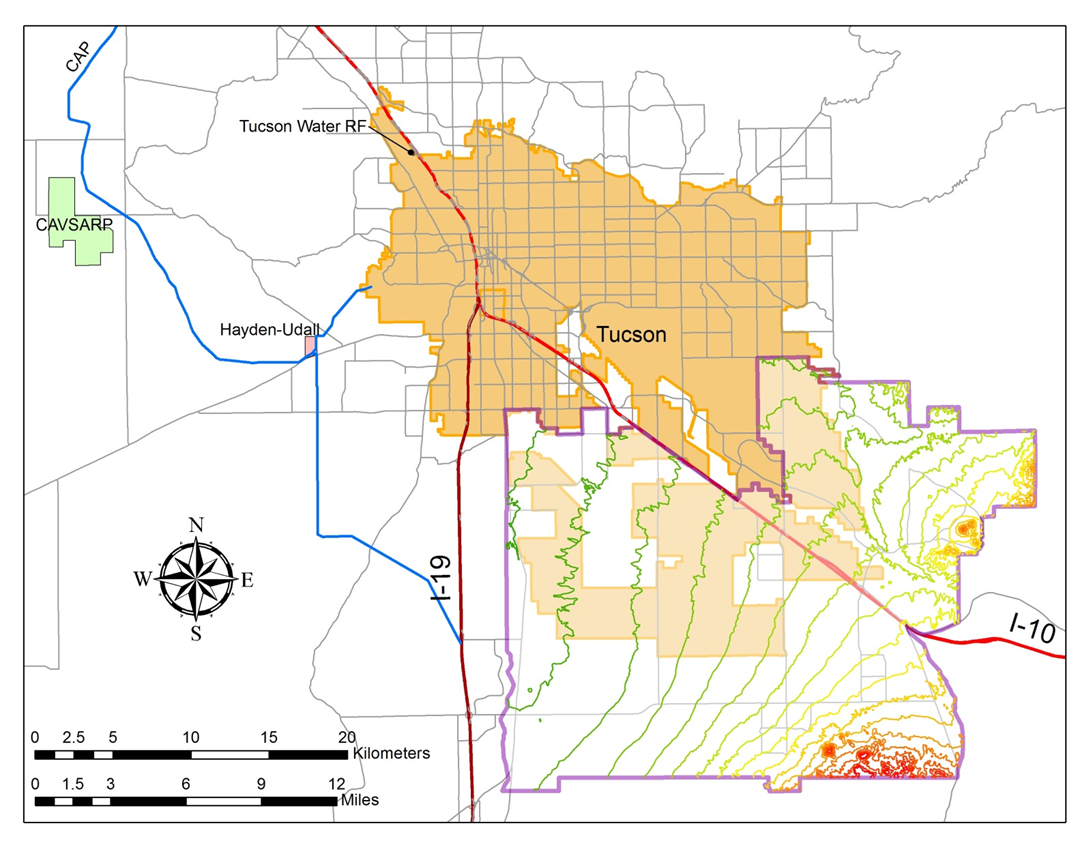
\includegraphics[width=.8\textwidth]{images/tucson_elevation}
	\caption{
		The southeastern region of Tucson considered in the water model, marked with a purple border.
	}
	\label{fig:tucson_map}
\end{figure}


\begin{table}[!ht]
	\centering
	\begin{tabular}{|c|cc||c|}
		\hline
		& \multicolumn{2}{|c||}{Population} & Supply \\
		Estimate & 2010 & 2050 & (CAP/yr) \\
		\hline
		\hline
		Low  & 33,304 & 371,804 & 130,000 \\
		\hline
		High & 40,705 & 762,427 & 140,000 \\
		\hline
	\end{tabular}\medskip
	\caption{
		Population of the southeastern region shown in Figure \ref{fig:tucson_map} in the low and high population estimates, along with the low and high estimates for amount of CAP water available per year.
		Note that the estimates for population and CAP availability are independent.
	}
	\label{tab:scenario_description}
\end{table}




\begin{figure}[!ht]
	\centering
	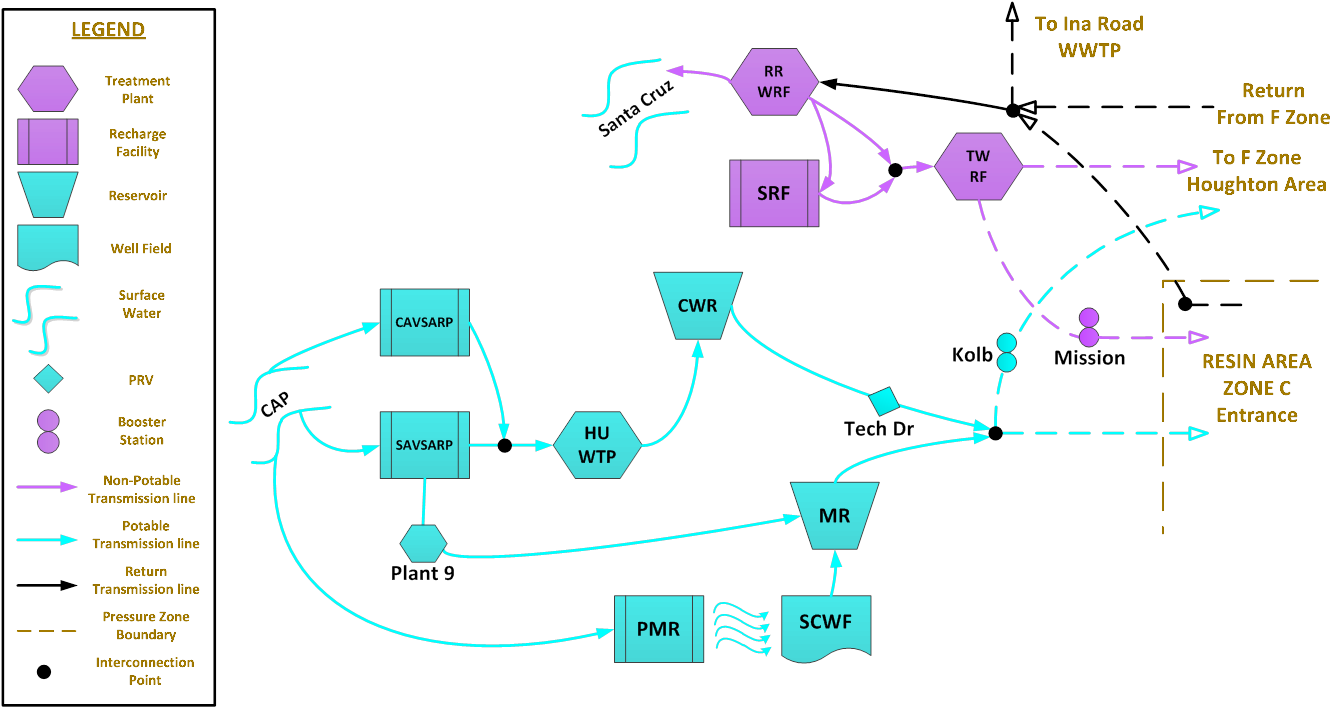
\includegraphics[width=.8\textwidth]{images/nodes_central}
	\caption{ (This figure is continued in Figures \ref{fig:zones_c_e} and \ref{fig:zones_split}, and Figure \ref{fig:zones_wwtp} provides a version with a decentralized treatment plant.)
		Network layout of the centralized water treatment system in Tucson.
		Nodes represent treatment facilities, reservoirs, etc.\ and arcs (arrows) represent transportation systems between nodes.\\ \\
		{\it Color coding:} blue represents potable water, purple shows nonpotable reclaimed water, and black shows wastewater.		\bigskip 
	}
	\label{fig:nodes_central}
\end{figure}

\bigskip 

\bigskip 

\begin{figure}[!hbpt]
	\centering
	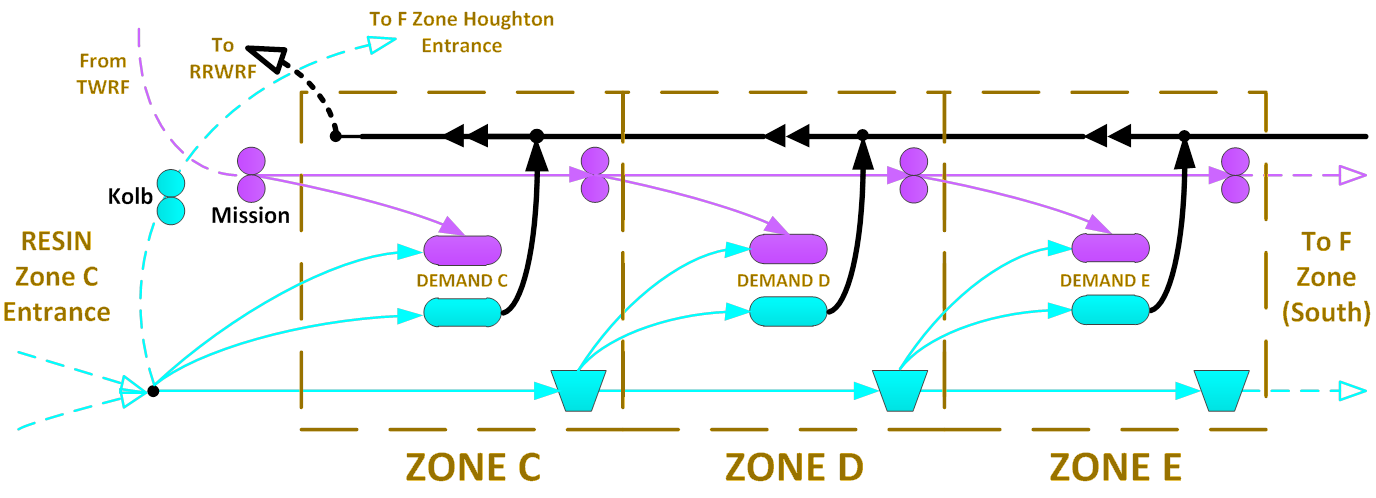
\includegraphics[width=.8\textwidth]{images/zones_c_e}
	\caption{
		Network layout of demand in elevation zones C--E of the southeastern region shown in Figure \ref{fig:tucson_map}.\bigskip 
	}
	\label{fig:zones_c_e}
\end{figure}

\bigskip 

\begin{figure}[!ht]
	\centering
	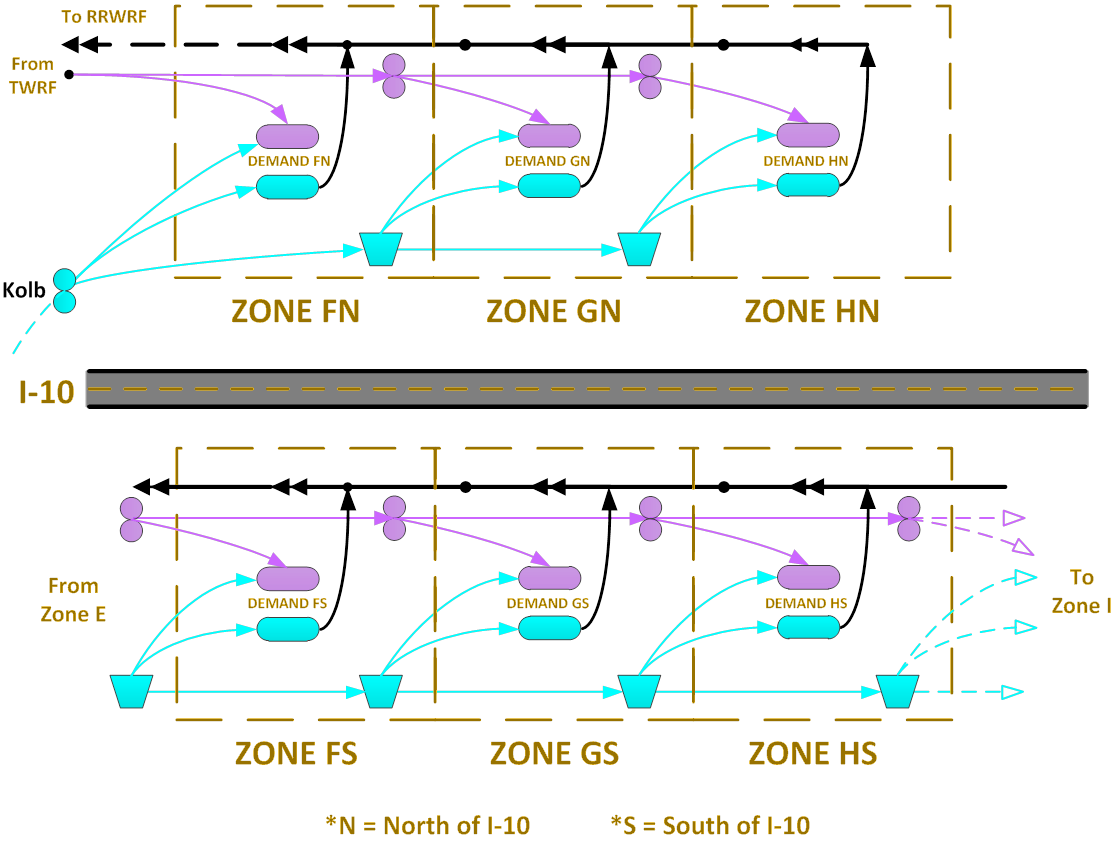
\includegraphics[width=.8\textwidth]{images/zones_split}
	\caption{
		Network layout of demand in elevation zones F--H of the southeastern region shown in Figure \ref{fig:tucson_map}.
		Highway I-10 splits these zones into north and south sections, with no water infrastructure crossing the highway.\bigskip 
	}
	\label{fig:zones_split}
\end{figure}

\bigskip

\bigskip 

\begin{figure}[!ht]
	\centering
	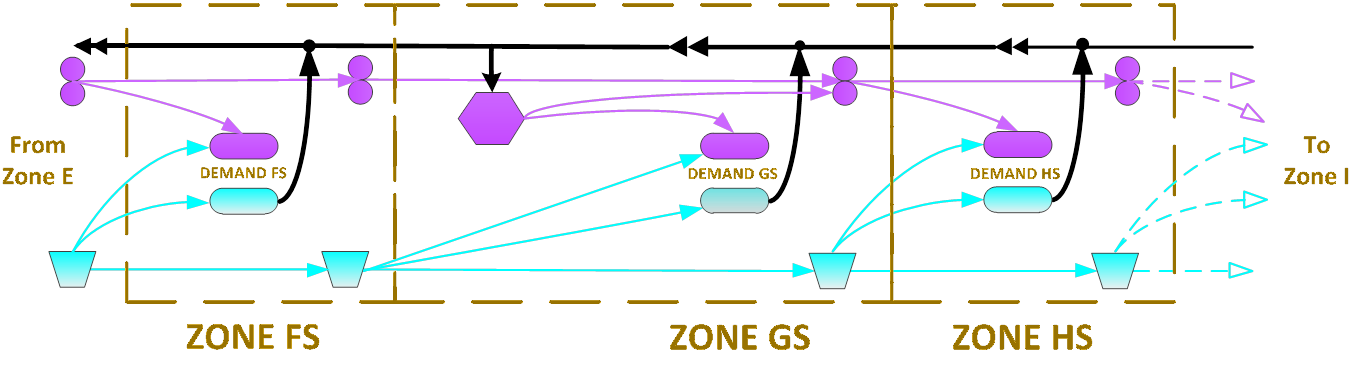
\includegraphics[width=.8\textwidth]{images/zones_south}
	\caption{
		Layout of south elevation zones F--H with a decentralized wastewater treatment plant in zone GS.\bigskip 
	}
	\label{fig:zones_wwtp}
\end{figure}

\FloatBarrier

%%%%%%%%%%%%%%%%%%%%%%%%%%%%%%%%%%%%%%%%%%%%%%%%%%%%%%%%%%%%%%%%%%%%%%%%%%%%%%%
\newpage
\FloatBarrier
\section{Figures for key findings}
\label{apx:results}
\FloatBarrier

\bigskip 

The figures in this appendix provide a summary of the key findings.


\begin{figure}[ht]
	\centering
	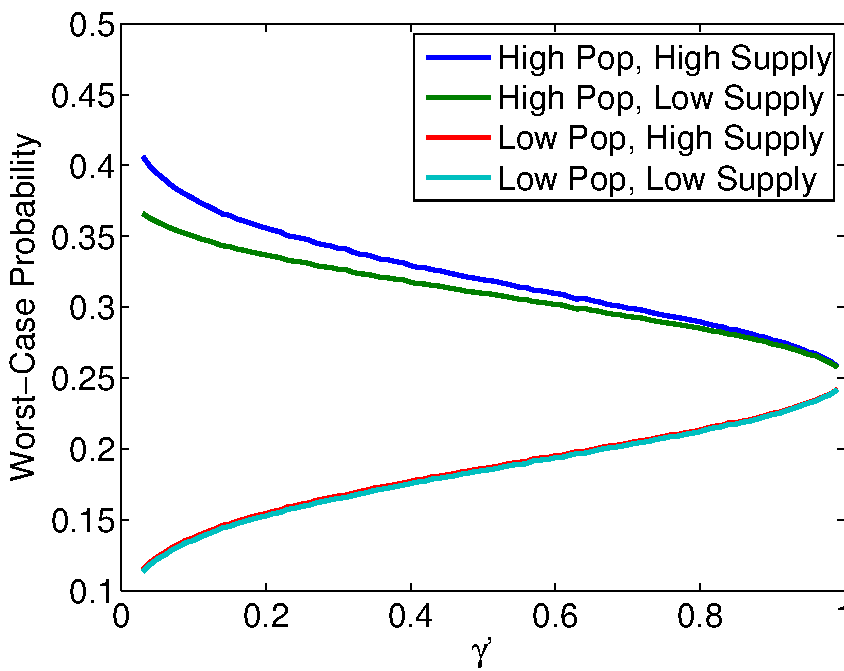
\includegraphics[width=.6\textwidth]{images/worst_case_probability}
	\caption{
		The probability of each of the four scenarios of the worst-case distribution for different values of the likelihood parameter $\gamma'$.
	}
	\label{fig:worst_case}
\end{figure}

\begin{figure}[hb]
	\centering
	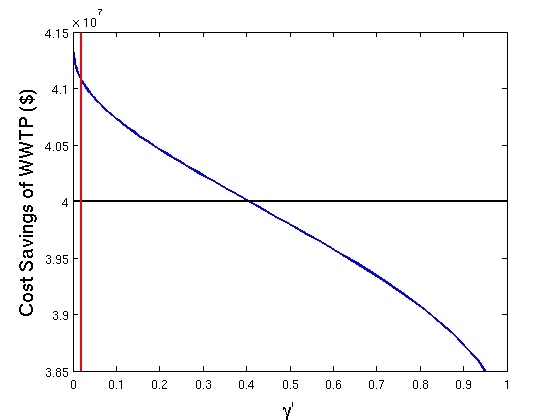
\includegraphics[width=.6\textwidth]{images/worst_case_cost_savings_3}
	\caption{
		Total savings on operating costs over 40 years from installing an additional wastewater treatment plant, depicted in Figure \ref{fig:zones_wwtp}.
		The cost of the plant is \$40 million, indicated by the black line.
		At the recommended likelihood parameter of $\gamma' = 0.02$, indicated by the red line, the additional wastewater treatment plant results in approximately \$1 million cost savings.
	}
	\label{fig:worst_case_savings}
\end{figure}

\end{document}
